\documentclass{standalone}
\usepackage{tikz}

\usetikzlibrary{matrix,positioning,shapes.arrows,fit}

\tikzset{ 
	table/.style={
		matrix of nodes,
		row sep=-\pgflinewidth,
		column sep=-\pgflinewidth,
		nodes={
			rectangle,draw,
			text width=0.5cm,
			align=center},
		text depth=0.125cm,
		text height=0.25cm,
		nodes in empty cells,
		outer sep=0cm,
	},
}

\begin{document}
	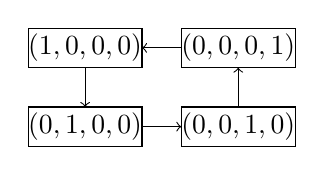
\begin{tikzpicture}[
		every node/.style = {
			draw, rectangle, 
			minimum width=0.75cm,
			minimum height=0.5cm,
			outer sep=0cm, inner sep=0cm,
			node distance=0cm
		}
		]
		\node (s1) {$(0, 0, 0, 1)$};
		\node [left=0.5cm of s1] (s8) {$(1, 0, 0, 0)$};
		\node [below=0.5cm of s8] (s4) {$(0, 1, 0, 0)$};
		\node [right=0.5cm of s4] (s2) {$(0, 0, 1, 0)$};
		\draw[->] (s1.west) -- (s8.east);
		\draw[->] (s8.south) -- (s4.north);
		\draw[->] (s4.east) -- (s2.west);
		\draw[->] (s2.north) -- (s1.south);
	\end{tikzpicture}
\end{document}